\section{Pipeline analítico paralelo}
\label{sec:pipeline-paralelo}

\subsection{Objetivo analítico y dataset}

El pipeline se orienta al objetivo analítico específico asignado al equipo ACC en la guía de la
Entrega 3: reincidencia de clientes y agrupamiento (\emph{clustering}) de incidencias. El dataset
sintético se genera con \texttt{spark/src/generate\_dataset.py} sobre 600{,}000 incidencias de
red, particionado en Parquet por zona geográfica, con dos características deliberadas necesarias
para que el análisis tenga señal real: el identificador de cliente (\texttt{client\_id}) se genera
con una distribución de Pareto en vez de uniforme —la mayoría de los clientes aparece una sola vez
y una minoría concentra muchas incidencias, reproduciendo el patrón real de reincidencia de un
ISP—, y cada incidencia incluye una descripción de texto libre corta generada por plantilla,
necesaria para la etapa de \emph{clustering} basada en texto. El carácter sintético del dataset y
la justificación de ambas decisiones de generación están documentados en el propio script y se
declaran también en \texttt{ai-usage-declaration.md}.

\subsection{Las cinco transformaciones}

\texttt{spark/src/transformations.py} implementa las cinco categorías de transformación exigidas
por la guía (Módulo E, Sección 5.6), aplicadas de forma no genérica al objetivo analítico del
equipo:

\begin{enumerate}[leftmargin=1.5em]
    \item \textbf{Filtrado (T1, sin \emph{shuffle})}: retiene únicamente incidencias resueltas y
        con los campos que el resto del pipeline necesita (\texttt{client\_id},
        \texttt{description} no nulos) — base válida tanto para el análisis de reincidencia como
        para el \emph{clustering}.
    \item \textbf{\emph{Join} colocalizado (T2, con \emph{shuffle})}: incidencias \emph{join}
        clientes por \texttt{client\_id}, instanciando la exigencia de colocalización de la
        Tabla 1 de la guía para el equipo ACC.
    \item \textbf{Función de ventana (T3, con \emph{shuffle})}: para cada cliente,
        \texttt{Window.partitionBy("client\_id")} \texttt{.orderBy("timestamp")} calcula el número de
        orden de cada incidencia (\texttt{incident\_seq}) y el \emph{timestamp} de la incidencia
        anterior del mismo cliente (\texttt{previous\_timestamp}) mediante \texttt{F.lag}.
    \item \textbf{Transformación de tipos temporales (T4, sin \emph{shuffle})}: a partir de
        \texttt{previous\_timestamp}, deriva la fecha de la incidencia, los días transcurridos
        desde la incidencia previa del cliente, y una bandera \texttt{is\_recurring\_30d} que
        marca reincidencia dentro de una ventana de 30 días — la métrica de reincidencia exigida
        para el equipo.
    \item \textbf{Aprendizaje automático (T5)}: agrupamiento de incidencias por texto y zona.
        La descripción libre se vectoriza con TF-IDF
        (\texttt{Tokenizer} + \texttt{StopWordsRemover} en español + \texttt{HashingTF} + \texttt{IDF}),
        la zona se codifica con \texttt{StringIndexer} (satisfaciendo también el ejemplo explícito
        de la guía), ambas \emph{features} se combinan con \texttt{VectorAssembler}, y se agrupan
        con \texttt{KMeans} ($k=5$, semilla fija 42 para reproducibilidad).
\end{enumerate}

\subsection{Ejecución y resultados observados}

El pipeline se ejecutó de extremo a extremo sobre el dataset completo de 600{,}000 filas mediante
un \emph{notebook} de Jupyter (\texttt{spark/notebooks/spark\_pipeline.ipynb}), exportado con
salidas reales vía \texttt{nbconvert --execute} para satisfacer el requisito de reproducibilidad —
no se trata de celdas de código estático sin ejecutar. La Tabla~\ref{tab:pipeline-resultados}
resume las cifras observadas en esa ejecución.

\begin{table}[H]
\centering
\caption{Resultados observados de la ejecución del pipeline sobre 600{,}000 filas}
\label{tab:pipeline-resultados}
\begin{tabular}{@{}lr@{}}
\toprule
\textbf{Magnitud} & \textbf{Valor} \\
\midrule
Filas totales del dataset & 600{,}000 \\
Filas tras T1 (filtrado, resueltas y completas) & 557{,}701 \\
Incidencias marcadas como reincidentes en 30 días (T4) & 380{,}753 (68.3\% de las filtradas) \\
\bottomrule
\end{tabular}
\end{table}

La alta proporción de reincidencia observada (68.3\%) es consistente con el diseño deliberado del
generador de datos: al concentrar una fracción significativa de las incidencias en un subconjunto
pequeño de clientes (distribución de Pareto), es esperable que buena parte de esas incidencias
caigan dentro de la ventana de 30 días de una incidencia previa del mismo cliente. La
Tabla~\ref{tab:clustering-resultados} muestra la distribución de tamaños de los cinco grupos
producidos por \texttt{KMeans} en T5.

\begin{table}[H]
\centering
\caption{Tamaño de los cinco grupos producidos por T5 (\emph{clustering})}
\label{tab:clustering-resultados}
\begin{tabular}{@{}rr@{}}
\toprule
\textbf{Grupo (\texttt{cluster})} & \textbf{Incidencias} \\
\midrule
0 & 13{,}761 \\
1 & 453{,}625 \\
2 & 27{,}815 \\
3 & 13{,}968 \\
4 & 48{,}532 \\
\bottomrule
\end{tabular}
\end{table}

La Figura~\ref{fig:resultados-spark} resume visualmente ambos resultados: el embudo de filtrado y
reincidencia, y la distribución de los cinco grupos de \emph{clustering}.

\begin{figure}[H]
\centering
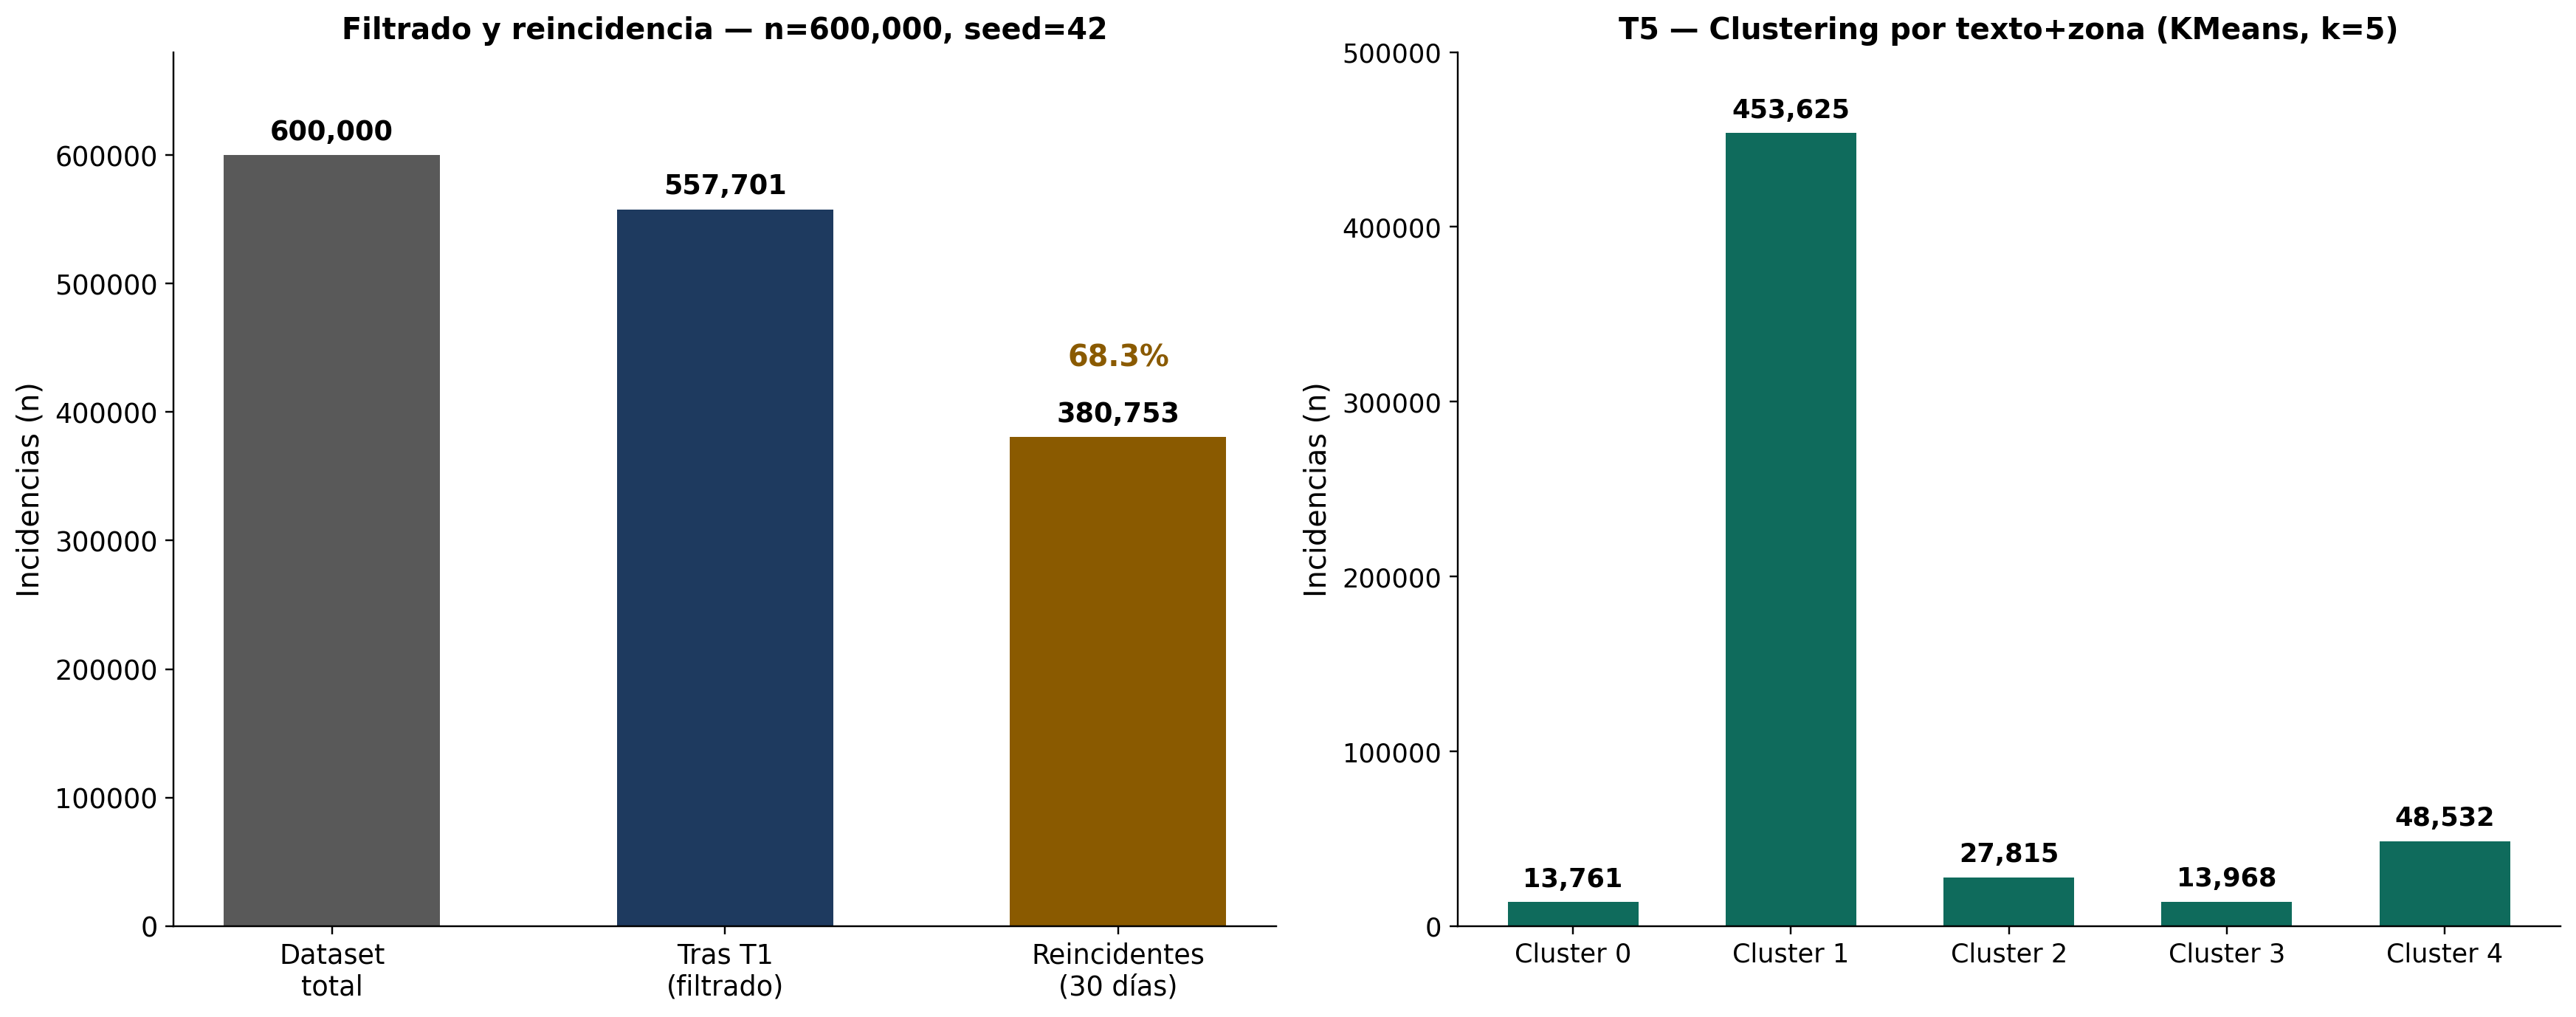
\includegraphics[width=0.95\textwidth]{figuras/resultados-pipeline-spark.png}
\caption{Izquierda: embudo de filtrado (T1) y reincidencia a 30 días (T4) sobre 600{,}000 filas,
ejecución única y determinista (\texttt{seed=42}). Derecha: distribución de los cinco grupos
producidos por \texttt{KMeans} en T5. Generado a partir de las salidas reales de
\texttt{spark\_pipeline.ipynb}.}
\label{fig:resultados-spark}
\end{figure}

La distribución de tamaños es marcadamente no uniforme, con un grupo dominante (cluster 1,
81.3\% de las filas filtradas) y cuatro grupos considerablemente más pequeños. Esto es coherente
con la naturaleza del \emph{feature} de texto: al usarse plantillas de descripción cortas y
relativamente similares entre sí para la mayoría de los tipos de incidencia comunes, es esperable
que el vector TF-IDF resultante concentre a la mayoría de las incidencias en una región densa del
espacio de \emph{features}, mientras que descripciones más específicas o zonas menos representadas
se separan en grupos más pequeños y homogéneos — un resultado no degenerado (no todos los puntos
en un único grupo, ni una partición trivialmente uniforme en cinco quintos iguales), suficiente
para ilustrar la mecánica de \emph{clustering} sobre datos reales del pipeline sin necesitar
afinar hiperparámetros adicionales fuera del alcance de esta entrega.

\subsection{Baseline secuencial}

Como contraparte de comparación para el protocolo experimental de la
Sección~\ref{sec:protocolo-resultados}, \texttt{spark/src/baseline.py} implementa las mismas cinco
transformaciones con pandas y scikit-learn puro, en un único proceso, sobre el mismo dataset. Este
baseline es el punto de referencia necesario para poder afirmar que el \emph{speedup} observado en
el pipeline de Spark proviene de paralelismo real y no únicamente del \emph{overhead} de
coordinación distribuida evitado por no usar Spark en absoluto para datasets de este tamaño.

Una ejecución individual de este baseline sobre las 600{,}000 filas (previa a las diez repeticiones
del protocolo formal de la Sección~\ref{sec:protocolo-resultados}) confirma su validez como
contraparte: reproduce exactamente las mismas 380{,}753 incidencias reincidentes obtenidas por el
pipeline de Spark, verificando que ambas implementaciones son equivalentes en resultado, no solo en
diseño. La Tabla~\ref{tab:baseline-tiempos} desglosa el tiempo de esta ejecución por transformación.

\begin{table}[H]
\centering
\caption{Tiempo por transformación del baseline secuencial en pandas (una ejecución, 600{,}000 filas)}
\label{tab:baseline-tiempos}
\begin{tabular}{@{}lr@{}}
\toprule
\textbf{Transformación} & \textbf{Tiempo (s)} \\
\midrule
Carga del Parquet & 1.55 \\
T1 — Filtrado & 0.86 \\
T2 — \emph{Join} con clientes & 0.74 \\
T3 — Función de ventana & 2.96 \\
T4 — Tipos temporales y bandera de reincidencia & 0.47 \\
T5 — \emph{Clustering} (TF-IDF + K-Means) & 36.88 \\
\midrule
\textbf{Total} & \textbf{43.46} \\
\bottomrule
\end{tabular}
\end{table}

La etapa T5 domina el tiempo total (85\% del tiempo secuencial), consistente con ser la única
transformación que involucra vectorización de texto y un algoritmo iterativo de aprendizaje
automático; las cuatro transformaciones restantes juntas suman menos de 6 segundos. Esta asimetría
anticipa que la fracción paralelizable relevante del pipeline se concentra en T5, un dato que se
retoma al ajustar la ley de Amdahl en la Sección~\ref{sec:protocolo-resultados}. Nótese también que
el \emph{clustering} de scikit-learn (baseline) y el de \texttt{pyspark.ml} producen distribuciones
de tamaño de grupo distintas entre sí (comparar con la Tabla~\ref{tab:clustering-resultados}):
ambas implementaciones usan K-Means con $k=5$ sobre \emph{features} equivalentes, pero difieren en
inicialización de centroides y en el algoritmo interno de vectorización TF-IDF, por lo que no se
espera —ni es necesario para la validez de la comparación de \emph{tiempos}— que sus asignaciones
de \emph{cluster} coincidan fila por fila.
